% Kompilácia: tectonic main.tex (alebo latexmk -xelatex main.tex).
\documentclass[12pt,a4paper]{article}
\usepackage{fontspec}
\usepackage{keyval}
\newcommand{\pksTinos}{\setmainfont{Tinos-Regular.ttf}[BoldFont=Tinos-Bold.ttf,ItalicFont=Tinos-Italic.ttf,BoldItalicFont=Tinos-BoldItalic.ttf]}
% Automatický výber: Times New Roman, Tinos, Liberation Serif.
\newcommand{\pksAutoFont}{%
  \IfFontExistsTF{Times New Roman}{\setmainfont{Times New Roman}}{%
    \IfFontExistsTF{Tinos-Regular.ttf}{\pksTinos}{\setmainfont{Liberation Serif}}}}
\newcommand{\pksSetFont}[1]{%
  \ifstrequal{#1}{auto}{\pksAutoFont}{%
    \ifstrequal{#1}{Tinos}{\pksTinos}{\setmainfont{#1}}}}
\usepackage{polyglossia}
\setdefaultlanguage{slovak}
\usepackage[left=25mm,right=25mm,top=32mm,bottom=22mm,headheight=42pt,headsep=9mm]{geometry}
\usepackage{graphicx,xcolor}
\usepackage{setspace,titlesec,fancyhdr,caption}
\usepackage[hidelinks,unicode]{hyperref}
\onehalfspacing
\setlength{\parindent}{0pt}
\setlength{\parskip}{6pt}
\setcounter{secnumdepth}{0}
\titleformat{\section}{\normalfont\fontsize{18}{22}\selectfont}{\thesection}{0pt}{}
\titleformat{\subsection}{\normalfont\fontsize{16}{20}\selectfont}{\thesubsection}{0pt}{}
\titleformat{\subsubsection}{\normalfont\fontsize{14}{18}\selectfont}{\thesubsubsection}{0pt}{}
\titlespacing*{\section}{0pt}{18pt}{10pt}
\titlespacing*{\subsection}{0pt}{14pt}{8pt}
\titlespacing*{\subsubsection}{0pt}{12pt}{6pt}
\DeclareCaptionFont{eleven}{\fontsize{11}{13}\selectfont}
\captionsetup{font=eleven,labelfont=normalfont,justification=centering}


% Údaje a voľba písma sa nastavujú v main.tex.
\newcommand{\nazovPrace}{Názov práce}
\newcommand{\nazovPredmetu}{Počítačové a komunikačné siete}
\newcommand{\autor}{Meno Priezvisko}
\newcommand{\aisid}{xxxxxx}
\newcommand{\veduci}{Meno Priezvisko}
\newcommand{\casCvicenia}{Deň xx:xx -- xx:xx}
\makeatletter
\define@key{pks}{title}{\renewcommand{\nazovPrace}{#1}}
\define@key{pks}{subject}{\renewcommand{\nazovPredmetu}{#1}}
\define@key{pks}{author}{\renewcommand{\autor}{#1}}
\define@key{pks}{ais-id}{\renewcommand{\aisid}{#1}}
\define@key{pks}{supervisor}{\renewcommand{\veduci}{#1}}
\define@key{pks}{class-time}{\renewcommand{\casCvicenia}{#1}}
\define@key{pks}{font}{\pksSetFont{#1}}
\newcommand{\pkssetup}[1]{\setkeys{pks}{#1}}
\makeatother
\pagestyle{fancy}
\fancyhf{}
\fancyhead[L]{\fontsize{12}{14}\selectfont\nazovPredmetu\\FIIT@STU\\\autor}
\fancyhead[R]{
\includegraphics[width=27mm]{template/assets/logo.png}}
\fancyfoot[C]{\fontsize{12}{14}\selectfont\thepage}
\renewcommand{\headrulewidth}{0pt}
\renewcommand{\footrulewidth}{0pt}


\newcommand{\pkstitlepage}{%
\hypersetup{pageanchor=false}
\begin{titlepage}
\newgeometry{left=25mm,right=25mm,top=18mm,bottom=12mm}
\thispagestyle{empty}
\begin{center}
{\fontsize{18}{22}\selectfont\bfseries Slovenská Technická Univerzita v Bratislave\par}
{\fontsize{14}{17}\selectfont Fakulta informatiky a informačných technológií\par}
\end{center}
\vspace*{81mm}
\begin{center}
{\fontsize{18}{22}\selectfont\bfseries\nazovPrace\par}
{\fontsize{14}{17}\selectfont\nazovPredmetu\par}
\vspace{7mm}
{\fontsize{14}{17}\selectfont\bfseries\autor\par}
{\fontsize{12}{15}\selectfont AIS ID: \aisid\par}
\end{center}
\vfill
{\singlespacing
\textbf{Vedúci cvičenia:} \veduci\\
\textbf{Čas cvičenia:} \casCvicenia\par}
\end{titlepage}
\restoregeometry
\setcounter{page}{1}
\hypersetup{pageanchor=true}

}

\newcommand{\pksdocument}{%
  \hypersetup{pdftitle={\nazovPrace},pdfauthor={\autor}}%
  \pkstitlepage
  \tableofcontents
  \newpage
}

\usepackage{amsmath}
\usepackage{tikz}
\usetikzlibrary{arrows.meta,positioning,shapes.geometric,calc}
\setlength{\emergencystretch}{1em}
\tikzset{
  every node/.style={execute at begin node=\setstretch{1}},
  flowbox/.style={draw,rounded corners,align=center,text width=6.6cm,minimum height=8mm,inner sep=5pt,font=\small},
  flowchoice/.style={draw,diamond,aspect=2.8,align=center,text width=3.2cm,inner sep=2pt,font=\small},
  flowend/.style={flowbox,fill=gray!10},
  flowarrow/.style={-{Latex},thick},
  seqactor/.style={draw,rounded corners,minimum width=2.5cm,minimum height=8mm,align=center,font=\small},
  seqarrow/.style={-{Latex},thick},
  seqnote/.style={draw,fill=gray!8,align=center,font=\small,inner sep=5pt}
}

\pkssetup{
  title={Komunikačný protokol pre IoT meteorologické zariadenia},
  subject={Počítačové a komunikačné siete},
  author={Sophie Hetešová},
  ais-id={141435},
  supervisor={Bc. Filip Hromada},
  class-time={Štvrtok -- 8:00},
  font={auto}, % Alternatívy: Tinos, Liberation Serif, Times New Roman (ak je nainštalované).
}

\let\originaltableofcontents\tableofcontents
\renewcommand{\tableofcontents}{\begingroup\small\singlespacing\originaltableofcontents\endgroup}

\begin{document}
\pksdocument

\section{Úvod a architektúra}

Riešenie prenáša merania vlastným binárnym protokolom nad UDP/IPv4, jednu správu na datagram. Zabezpečuje registráciu, potvrdenie, integritu a dostupnosť senzorov. Pôvodná JSON verzia zostáva v \texttt{json\_baseline/} na porovnanie.

\texttt{server.py} spravuje relácie a merania. \texttt{tester.py} emuluje štyri typy senzorov; každý má vlastné vlákno, UDP socket, frontu a časovače. Menu odovzdáva príkazy cez fronty, takže senzory fungujú nezávisle. Server má jednu sieťovú slučku a samostatné menu. \texttt{lib.py} poskytuje validáciu a logovanie; \path{binary_protocol.py} kódovanie a \path{wire_protocol.py} prepojenie formátu s reláciami.

Spustenie: \texttt{python3 server.py} a \texttt{python3 tester.py}. IP a port sa zadávajú v rozhraní (predvolene 127.0.0.1:9000). Sockety sa vytvárajú priamo knižnicou \texttt{socket}.

Konzolové logy zapína \texttt{--console-logs}. Osem senzorov spustí voľba \texttt{--sensors-per-type} s argumentom \texttt{2}.

Menu testera: 1 vlastné meranie, 2 poškodenie DATA, 3 automatika, 4 odpojenie, 5 registrácia, 0 koniec. Menu servera: 1 potláčanie ACK, 2 prehľad relácií (stav, vek merania, zostávajúce potlačené ACK), 0 koniec.

\subsection{Použité knižnice}

Server a tester používajú štandardnú knižnicu Pythonu. Meracie skripty navyše používajú Matplotlib na grafy a externé nástroje TShark/dumpcap na analýzu a zachytávanie:
\begin{center}
\small\singlespacing
\begin{tabular}{p{6cm} p{7cm}}
\hline
\textbf{Moduly} & \textbf{Úloha} \\
\hline
\texttt{socket} & UDP komunikácia. \\
\texttt{threading}, \texttt{queue} & Vlákna a odovzdávanie príkazov. \\
\texttt{json}, \texttt{zlib} & Čitateľné logy, JSON porovnanie a CRC32. \\
\texttt{ipaddress}, \texttt{decimal} & Validácia adries a číselných vstupov. \\
\texttt{secrets}, \texttt{random}, \texttt{copy} & Tokeny, náhodné merania a poškodená kópia. \\
\texttt{struct}, \texttt{argparse} & Binárne polia a voľby spustenia. \\
\texttt{time}, \texttt{logging} & Časovače a logovanie. \\
\texttt{os}, \texttt{sys}, \texttt{shutil}, \texttt{readline} & Terminál; \texttt{readline} je voliteľný. \\
\hline
\end{tabular}
\end{center}

Meracie nástroje ďalej používajú štandardné moduly \texttt{csv}, \texttt{pathlib}, \texttt{hashlib}, \texttt{statistics}, \texttt{subprocess}, \texttt{signal} a \texttt{collections}. Testy používajú \texttt{unittest}, mock objekty a dočasné súbory. Matplotlib je potrebný iba pre meracie grafy; pre server a tester sa externé Python balíky neinštalujú.

Logy udalostí (SYSTEM) a prenosov (MESSAGE) sa zapisujú do \texttt{server.log} a \texttt{tester.log}; pri novom spustení sa prepíšu. Súbor zachováva celý obsah správ a formát \texttt{čas | typ | úroveň | zdroj | udalosť}. Čas je UTC s milisekundami. Súborový zápis je vždy zapnutý. Voľba \texttt{--console-logs} zapne aj konzolové bloky s jednotkami; farby závisia od terminálu. Polia \texttt{sensor\_id} a \texttt{ack\_for} môžu byť v logu odvodené zo stavu relácie, hoci sa v binárnom pakete neprenášajú samostatne.

\section{Návrh protokolu}

\subsection{Relácia a pôvodný JSON návrh}

REGISTER obsahuje typ a jedinečné ID senzora. Server uloží jeho zdrojovú IP adresu a port a pridelí token: osem náhodných bajtov zapísaných ako 16 hexadecimálnych znakov. V binárnom prenose sa ID posiela iba pri registrácii; následne sa relácia určuje tokenom, typom senzora a zdrojovou adresou. Token je v pakete osem bajtov, v logu 16 hexadecimálnych znakov. Server nepridelí nulu ani token existujúcej relácie. Po zrušení relácie token prestáva platiť. Nasledujúce JSON polia a príklady zachytávajú pôvodný návrh, nie finálnu prenosovú reprezentáciu.

V pôvodnom JSON návrhu mal server vlastný čítač a odpovede používali \texttt{ack\_for}. Vo finálnom formáte odpoveď zopakuje \texttt{seq} požiadavky; retransmisia zachová číslo aj pôvodné bajty. Každý senzor má nezávislý čítač od 1. Pred vyčerpaním 32 bitov sa musí relácia obnoviť; automatické obnovenie pri tomto limite zatiaľ nie je implementované.

\subsection{JSON správy a príklady pôvodného návrhu}

Príklady používajú ukážkový token. Zalomenia slúžia na čitateľnosť; JSON baseline posiela objekty bez nadbytočných medzier. Binárna verzia odlišuje registračné potvrdenie REGISTER\_ACK od dátového ACK.

\paragraph{REGISTER -- senzor $\rightarrow$ server.}
Žiadosť o registráciu typu a ID. Už obsadené ID sa odmietne.
\begin{quote}\begin{minipage}{\linewidth}\small\singlespacing
\begin{verbatim}
{"type":"REGISTER","seq":1,"sensor_type":"ThermoNode",
 "sensor_id":"T-01"}
\end{verbatim}
\end{minipage}\end{quote}

\paragraph{ACK -- server $\rightarrow$ senzor.}
Potvrdzuje registráciu alebo platné meranie. Token sa pridáva iba pri registrácii.
\begin{quote}\begin{minipage}{\linewidth}\small\singlespacing
\begin{verbatim}
{"type":"ACK","seq":1,"ack_for":1,
 "token":"a1b2c3d4e5f60718"}
{"type":"ACK","seq":2,"ack_for":2}
\end{verbatim}
\end{minipage}\end{quote}

\paragraph{DATA -- senzor $\rightarrow$ server.}
Automatické aj ručné meranie majú rovnaký formát. Objekt \texttt{values} obsahuje parametre registrovaného typu.
\begin{quote}\begin{minipage}{\linewidth}\small\singlespacing
\begin{verbatim}
{"type":"DATA","seq":2,"sensor_id":"T-01",
 "token":"a1b2c3d4e5f60718","values":{
 "temperature":21.3,"humidity":55.4,
 "dew_point":11.9,"pressure":1013.25},"crc":1819254021}
\end{verbatim}
\end{minipage}\end{quote}

\paragraph{RETRANSMIT -- server $\rightarrow$ senzor.}
Pri chybnom CRC server vyžiada správny originál. Tester overí reláciu a znova odošle tú istú DATA s rovnakým \texttt{seq}, hodnotami a CRC. Limit sú tri odoslania vrátane pôvodného.
\begin{quote}\begin{minipage}{\linewidth}\small\singlespacing
\begin{verbatim}
{"type":"RETRANSMIT","seq":3,"ack_for":2,
 "sensor_id":"T-01","token":"a1b2c3d4e5f60718",
 "reason":"Integrity check failed"}
\end{verbatim}
\end{minipage}\end{quote}

\paragraph{REJECT -- server $\rightarrow$ senzor.}
Odmietnutie napríklad pri neplatnom tokene, obsadenom ID alebo hodnotách mimo rozsahu.
\begin{quote}\begin{minipage}{\linewidth}\small\singlespacing
\begin{verbatim}
{"type":"REJECT","seq":4,"ack_for":2,
 "reason":"Invalid sensor ID or token"}
\end{verbatim}
\end{minipage}\end{quote}

\paragraph{KEEPALIVE -- server $\rightarrow$ senzor.}
Overuje dostupnosť senzora, od ktorého neprichádzajú merania.
\begin{quote}\begin{minipage}{\linewidth}\small\singlespacing
\begin{verbatim}
{"type":"KEEPALIVE","seq":5,"sensor_id":"T-01",
 "token":"a1b2c3d4e5f60718"}
\end{verbatim}
\end{minipage}\end{quote}

\paragraph{KEEPALIVE\_ACK -- senzor $\rightarrow$ server.}
Odpoveď na konkrétnu sondu; posiela sa aj pri vypnutej automatike.
\begin{quote}\begin{minipage}{\linewidth}\small\singlespacing
\begin{verbatim}
{"type":"KEEPALIVE_ACK","seq":3,"ack_for":5,
 "sensor_id":"T-01","token":"a1b2c3d4e5f60718"}
\end{verbatim}
\end{minipage}\end{quote}

\subsection{Parametre senzorov}

Obe hranice rozsahov sú povolené. Uvedená desatinná presnosť je maximálna; celočíselné polia sa prijímajú iba ako celé čísla. Tester aj server hodnoty validujú. Neplatný vstup možno opraviť bez pádu programu.

\begin{center}
\small\singlespacing
\begin{tabular}{p{5.3cm} p{4.2cm} p{3.2cm}}
\hline
\textbf{Parameter} & \textbf{Rozsah} & \textbf{Presnosť} \\
\hline
\multicolumn{3}{l}{\textbf{ThermoNode}} \\
\texttt{temperature} & $-50{,}0$ až $60{,}0$~°C & 1 desatinné miesto \\
\texttt{humidity} & $0{,}0$ až $100{,}0$~\% & 1 desatinné miesto \\
\texttt{dew\_point} & $-50{,}0$ až $60{,}0$~°C & 1 desatinné miesto \\
\texttt{pressure} & $800{,}00$ až $1100{,}00$~hPa & 2 desatinné miesta \\
\hline
\multicolumn{3}{l}{\textbf{WindSense}} \\
\texttt{wind\_speed} & $0{,}0$ až $50{,}0$~m/s & 1 desatinné miesto \\
\texttt{wind\_gust} & $0{,}0$ až $70{,}0$~m/s & 1 desatinné miesto \\
\texttt{wind\_direction} & 0 až 359 stupňov & celé číslo \\
\texttt{turbulence} & $0{,}0$ až $1{,}0$ & 1 desatinné miesto \\
\hline
\multicolumn{3}{l}{\textbf{RainDetect}} \\
\texttt{rainfall} & $0{,}0$ až $500{,}0$~mm & 1 desatinné miesto \\
\texttt{soil\_moisture} & $0{,}0$ až $100{,}0$~\% & 1 desatinné miesto \\
\texttt{flood\_risk} & 0 až 3 & celé číslo \\
\texttt{rain\_duration} & 0 až 60 minút & celé číslo \\
\hline
\multicolumn{3}{l}{\textbf{AirQuality}} \\
\texttt{co2} & 300 až 5000 ppm & celé číslo \\
\texttt{ozone} & $0{,}0$ až $500{,}0$~µg/m\textsuperscript{3} & 1 desatinné miesto \\
\texttt{air\_quality\_index} & 0 až 500 & celé číslo \\
\hline
\end{tabular}
\end{center}


\clearpage
\subsection{Binárny formát v1}

Všetky viacbajtové celé čísla sú v sieťovom poradí (big-endian). Bajty sa čítajú od začiatku datagramu; bity v payload poli od najvyššieho bitu. Datagram neobsahuje dĺžkové pole, jeho presná veľkosť vyplýva z typu správy a senzora. Neposiela sa čas merania; UTC čas vzniká pri logovaní.

\begin{figure}[!htbp]
\centering
\begin{tikzpicture}[x=1cm,y=1cm,font=\small]
\draw[fill=blue!8] (0,0) rectangle (2,0.8);
\draw[fill=blue!8] (2,0) rectangle (6,0.8);
\draw[fill=blue!8] (6,0) rectangle (12,0.8);
\node at (1,0.4) {Riadenie 1 B};
\node at (4,0.4) {Sekvencia 4 B};
\node at (9,0.4) {Token 8 B};
\draw (0,-1.2) rectangle (8.5,-0.4);
\draw[fill=gray!15] (8.5,-1.2) rectangle (12,-0.4);
\node at (4.25,-0.8) {Payload: 0 B alebo podľa správy};
\node at (10.25,-0.8) {CRC32 4 B};
\node[align=center] at (6,-1.9) {Riadiaci bajt od najvyššieho bitu: 7--6 verzia,\\5--3 typ správy, 2--1 senzor, 0 rezerva};
\end{tikzpicture}

\caption{Hlavička, payload a CRC binárneho datagramu.}
\end{figure}

\begin{center}\small\singlespacing
\begin{tabular}{p{2.8cm} p{2cm} p{8cm}}
\hline Pole & Offset & Význam \\\hline
Riadiaci bajt & 0 & Bity 7--6: verzia 01; 5--3: typ správy; 2--1: senzor; bit 0: rezerva 0. \\
\texttt{seq} & 1--4 & uint32, rozsah 1 až $2^{32}-1$; odpoveď opakuje číslo požiadavky. \\
\texttt{token} & 5--12 & uint64; nula pri REGISTER a odmietnutí neplatnej/neexistujúcej relácie. \\
Payload & od 13 & Dĺžka závisí od typu; môže byť prázdny. \\
CRC32 & posledné 4 B & Súčet celej hlavičky a payloadu. \\\hline
\end{tabular}\end{center}

Typy senzorov: 00 ThermoNode, 01 WindSense, 10 RainDetect, 11 AirQuality. Pevná réžia datagramu je 17 B. ACK sa priraďuje podľa socketu, typu senzora, tokenu a čakajúceho \texttt{seq}; \texttt{ack\_for} v pakete nie je. KEEPALIVE má samostatné číslo sondy servera, KEEPALIVE\_ACK ho zopakuje.

\begin{center}\small\singlespacing
\begin{tabular}{c l p{6.5cm} l}
\hline Kód & Typ & Payload & Celkom \\\hline
000 & REGISTER & uint8 dĺžka $N$ a $N$ UTF-8 bajtov ID & $18+N$ B \\
001 & ACK & bez payloadu & 17 B \\
010 & REJECT & uint8 kód dôvodu & 18 B \\
011 & DATA & hodnoty podľa typu senzora & 21--23 B \\
100 & RETRANSMIT & bez payloadu & 17 B \\
101 & KEEPALIVE & bez payloadu & 17 B \\
110 & KEEPALIVE\_ACK & bez payloadu & 17 B \\
111 & REGISTER\_ACK & nový token v hlavičke & 17 B \\\hline
\end{tabular}\end{center}

ID má 1--255 UTF-8 bajtov, nesmie byť prázdne ani tvorené iba medzerami. REGISTER\_ACK musí obsahovať nenulový token. REJECT pri registrácii má token nula. Dôvody odmietnutia: 1 neplatná relácia/token, 2 obsadené ID, 3 neplatné hodnoty, 4 nepodporovaná správa/verzia, 5 konflikt sekvencie, 6 nesprávna zdrojová adresa. Dekóder kontroluje aj rezervný bit, presnú dĺžku, UTF-8 a nulové doplnenie. Pri neinterpretovateľnom datagrame sa chyba zaloguje bez odpovede; nie každá chyba vyvolá REJECT.

\subsection{Bitové kódovanie hodnôt}

Pre minimum $m$ a počet desatinných miest $d$ je kód
\[
 k=(v-m)10^d,\qquad v=m+\frac{k}{10^d}.
\]
Výpočet používa presné desatinné hodnoty; nepovolená presnosť sa odmieta, nezaokrúhľuje. Počet bitov je $\lceil\log_2(K+1)\rceil$, kde $K=(M-m)10^d$. Napríklad 21,3~°C sa pri minime $-50$~°C uloží ako 713 do 11 bitov. Nepoužité kódy nad maximom sú neplatné.

\begin{center}\small\singlespacing
\begin{tabular}{l l r r}
\hline Senzor & Polia v poradí prenosu & Bity & Max. kód \\\hline
ThermoNode & temperature & 11 & 1100 \\
 & humidity & 10 & 1000 \\
 & dew\_point & 11 & 1100 \\
 & pressure & 15 & 30000 \\\hline
WindSense & wind\_speed & 9 & 500 \\
 & wind\_gust & 10 & 700 \\
 & wind\_direction & 9 & 359 \\
 & turbulence & 4 & 10 \\\hline
RainDetect & rainfall & 13 & 5000 \\
 & soil\_moisture & 10 & 1000 \\
 & flood\_risk & 2 & 3 \\
 & rain\_duration & 6 & 60 \\\hline
AirQuality & co2 & 13 & 4700 \\
 & ozone & 13 & 5000 \\
 & air\_quality\_index & 9 & 500 \\\hline
\end{tabular}\end{center}

Polia sú spojené bez medzier. Na konci sa pridá nulové doplnenie do celého bajtu. ThermoNode má 47 bitov + 1 nulu (6 B), WindSense 32 bitov (4 B), RainDetect 31 bitov + 1 nulu (4 B), AirQuality 35 bitov + 5 núl (5 B). Celé DATA majú postupne 23, 21, 21 a 22 B. Názvy parametrov, ID a desatinné bodky sa v DATA neprenášajú.

\subsection{Integrita a časovanie}

V binárnej verzii pokrýva \texttt{zlib.crc32()} všetky bajty pred poslednými štyrmi bajtmi CRC: riadiaci bajt, sekvenciu, token aj payload. Výsledok sa uloží ako neznamienkový uint32 v big-endian poradí. Kontrola platí pre všetky typy správ. CRC odhaľuje náhodné poškodenie, neposkytuje autentifikáciu ani šifrovanie. V pôvodnej JSON verzii sa CRC počítalo nad kanonickým JSON objektom bez poľa \texttt{crc}.

Pri simulácii chyby tester zmení hodnotu odosielanej kópie a zachová pôvodné CRC. Uložený správny paket zostane dostupný na opakovanie. Server pri poškodení žiada RETRANSMIT iba pri priraditeľnej relácii a správnej zdrojovej adrese; neplatné hlavičky alebo neznáme relácie sa nesmú považovať za dôveryhodné.

Prvá DATA sa odošle po registrácii, ďalšie každých 10 s. Ručné meranie nemení plán automatiky. Bez ACK do 3 s tester zopakuje rovnaké binárne bajty; celkovo najviac tri odoslania. Po ďalších 3 s od posledného pokusu správu zahodí. Do limitu sa započítava aj opakovanie na RETRANSMIT. Server potvrdí platnú duplicitu, ale nezapíše ju ako nové meranie. Uchováva najviac 256 nedávnych sekvencií na reláciu. Konflikt rovnakého čísla s iným CRC odmietne a neobnoví ním časovač.

Po 15 s bez DATA server vypíše SENSOR IDLE a pošle KEEPALIVE. Bez odpovedí nasledujú sondy v 20. a 25. sekunde a zrušenie relácie v 30. sekunde s výpisom SENSOR DISCONNECTED. Ak DATA ešte neprišla, čas sa počíta od registrácie. KEEPALIVE\_ACK vynuluje počet nezodpovedaných sond, nová DATA obnoví aktívny stav.

Lokálny časovač senzora je 30 s od platného kontaktu: KEEPALIVE, ACK merania alebo RETRANSMIT. Vypnutie automatiky nebráni odpovediam na sondy; úplné odpojenie áno. Po zániku relácie nová registrácia pridelí nový token. Časovanie používa \texttt{time.monotonic()}.

\clearpage
\section{Komunikačné cykly}

\subsection{Prijímanie na serveri}

Server strieda obsluhu príkazov, časovačov a príjem UDP. Podľa typu správy overí registráciu, meranie alebo odpoveď na sondu a aktualizuje reláciu (obrázok~\ref{fig:server-receive}). Chybný binárny formát sa zaloguje a zahodí; pri priraditeľnej poškodenej DATA sa vyžiada oprava. Timeout socketu je najviac 0,2 s, aby kontroly fungovali aj bez prijatých správ.

\begin{figure}[!htbp]
\centering
\begin{tikzpicture}[node distance=6mm]
\node[flowend] (start) {Opakovanie hlavnej slučky servera};
\node[flowbox,below=of start] (timers) {Príkazy menu a kontrola časovačov relácií};
\node[flowbox,below=of timers] (receive) {Prijať UDP datagram cez \texttt{recvfrom()}};
\node[flowchoice,below=of receive] (valid) {Platný binárny formát?};
\node[flowbox,right=12mm of valid,text width=2.5cm] (discard) {Zalogovať chybu a zahodiť};
\node[flowbox,below=8mm of valid] (dispatch) {REGISTER: overiť typ a ID\\DATA: relácia, adresa, CRC, hodnoty a duplicity\\KEEPALIVE\_ACK: overiť čakajúcu sondu};
\node[flowbox,below=of dispatch] (state) {Aktualizovať platnú reláciu alebo pripraviť odmietnutie};
\node[flowbox,below=of state] (reply) {Ak treba odpoveď, vykonať odosielací cyklus};
\node[flowend,below=of reply] (repeat) {Ďalšia iterácia};
\draw[flowarrow] (start)--(timers);
\draw[flowarrow] (timers)--(receive);
\draw[flowarrow] (receive)--(valid);
\draw[flowarrow] (valid)--node[above,font=\small]{nie}(discard);
\draw[flowarrow] (valid)--node[right,font=\small]{áno}(dispatch);
\draw[flowarrow] (dispatch)--(state);
\draw[flowarrow] (state)--(reply);
\draw[flowarrow] (reply)--(repeat);
\draw[flowarrow] (discard.south)|-(repeat.east);
\draw[flowarrow] (repeat.west)--++(-10mm,0)|-(start.west);
\end{tikzpicture}

\caption{Prijímací cyklus servera.}
\label{fig:server-receive}
\end{figure}

\clearpage
\subsection{Odosielanie na serveri}

Odpoveď vzniká pri spracovaní správy alebo časovača. Server zostaví odpoveď s číslom požiadavky alebo novú sondu so samostatným číslom, doplní CRC, zakóduje binárne polia a odošle datagram na adresu senzora (obrázok~\ref{fig:server-send}). Pri KEEPALIVE uloží číslo sondy a termín ďalšej kontroly. Odosielanie je súčasťou hlavnej slučky.

\begin{figure}[!htbp]
\centering
\begin{tikzpicture}[node distance=7mm]
\node[flowend] (start) {Výsledok spracovania správy alebo časovača};
\node[flowchoice,below=of start] (needed) {Treba odpoveď a ACK nie je potlačené?};
\node[flowbox,right=12mm of needed,text width=2.5cm] (none) {Bez odpovede};
\node[flowbox,below=8mm of needed] (build) {Zostaviť REGISTER\_ACK, ACK, REJECT, RETRANSMIT alebo KEEPALIVE};
\node[flowbox,below=of build] (seq) {Odpoveď: zopakovať \texttt{seq} požiadavky; sonda: nové číslo; doplniť token a typ senzora};
\node[flowbox,below=of seq] (encode) {Zakódovať binárnu hlavičku a payload; doplniť CRC32};
\node[flowbox,below=of encode] (send) {Odoslať cez \texttt{sendto()} na adresu senzora};
\node[flowbox,below=of send] (log) {Zalogovať odoslaný obsah; pri sonde uložiť jej číslo a ďalší termín};
\node[flowend,below=of log] (end) {Návrat do hlavnej slučky};
\draw[flowarrow] (start)--(needed);
\draw[flowarrow] (needed)--node[above,font=\small]{nie}(none);
\draw[flowarrow] (needed)--node[right,font=\small]{áno}(build);
\draw[flowarrow] (build)--(seq);
\draw[flowarrow] (seq)--(encode);
\draw[flowarrow] (encode)--(send);
\draw[flowarrow] (send)--(log);
\draw[flowarrow] (log)--(end);
\draw[flowarrow] (none.south)|-(end.east);
\end{tikzpicture}

\caption{Odosielací cyklus servera.}
\label{fig:server-send}
\end{figure}

\clearpage
\subsection{Odosielanie vo vlákne senzora}

Vlákno spracuje príkazy svojej fronty a plán automatických meraní. Pri novej DATA doplní CRC a uchová správny originál. Pri retransmisii použije pôvodné číslo aj obsah (obrázok~\ref{fig:tester-send}). Menu so socketom nepracuje.

\begin{figure}[!htbp]
\centering
\begin{tikzpicture}[node distance=6mm]
\node[flowend] (start) {Príkaz menu, automatické meranie, RETRANSMIT alebo 3 s bez ACK (najviac 3 odoslania)};
\node[flowchoice,below=of start] (allowed) {Akcia je povolená v aktuálnom stave?};
\node[flowbox,right=12mm of allowed,text width=2.5cm] (invalid) {Zalogovať odmietnutú akciu};
\node[flowbox,below=8mm of allowed] (build) {Zostaviť REGISTER, DATA alebo KEEPALIVE\_ACK; pri oprave použiť uložený originál};
\node[flowbox,below=of build] (crc) {Pri novej DATA vypočítať binárne CRC32 a uložiť správny paket};
\node[flowbox,below=of crc] (corrupt) {Ak bola zvolená simulácia chyby, zmeniť iba odosielanú kópiu DATA};
\node[flowbox,below=of corrupt] (send) {Odoslať binárny paket vlastným socketom; pri opakovaní identické bajty; zalogovať obsah};
\node[flowbox,below=of send] (pending) {Pri REGISTER a DATA uložiť čakanie na odpoveď; aktualizovať plán merania};
\node[flowend,below=of pending] (end) {Pokračovať v slučke senzora};
\draw[flowarrow] (start)--(allowed);
\draw[flowarrow] (allowed)--node[above,font=\small]{nie}(invalid);
\draw[flowarrow] (allowed)--node[right,font=\small]{áno}(build);
\draw[flowarrow] (build)--(crc);
\draw[flowarrow] (crc)--(corrupt);
\draw[flowarrow] (corrupt)--(send);
\draw[flowarrow] (send)--(pending);
\draw[flowarrow] (pending)--(end);
\draw[flowarrow] (invalid.south)|-(end.east);
\end{tikzpicture}

\caption{Odosielací cyklus jedného senzora.}
\label{fig:tester-send}
\end{figure}

\clearpage
\subsection{Prijímanie vo vlákne senzora}

Senzor prijíma iba odpovede zo zadanej adresy servera. REGISTER\_ACK vytvorí reláciu, dátové ACK ukončí čakanie, RETRANSMIT vyžiada odoslanie originálu a KEEPALIVE sa potvrdí aj pri vypnutých meraniach (obrázok~\ref{fig:tester-receive}). REJECT ukončí požiadavku; odmietnutie tokenu aj lokálnu reláciu. Pri ukončení testera sa zastavia všetky vlákna a zatvoria sockety.

\begin{figure}[!htbp]
\centering
\begin{tikzpicture}[node distance=6mm]
\node[flowend] (start) {Opakovanie slučky jedného senzora};
\node[flowbox,below=of start] (timers) {Spracovať frontu príkazov a časovače; pri chýbajúcom ACK celkovo najviac 3 odoslania, potom zahodiť; relácia bez kontaktu 30 s zaniká};
\node[flowbox,below=of timers] (receive) {Čakať na datagram najviac 0,2 s alebo do najbližšieho termínu};
\node[flowchoice,below=of receive] (valid) {Prišla použiteľná správa od servera?};
\node[flowbox,right=12mm of valid,text width=2.5cm] (ignore) {Timeout alebo zahodenie správy};
\node[flowbox,below=8mm of valid] (dispatch) {REGISTER\_ACK: vytvoriť reláciu\\ACK: potvrdiť čakajúce meranie\\RETRANSMIT: overiť reláciu a odoslať originál\\KEEPALIVE: overiť reláciu a odpovedať\\REJECT: ukončiť príslušné čakanie};
\node[flowbox,below=of dispatch] (state) {Aktualizovať stav senzora a čas platného kontaktu podľa typu odpovede};
\node[flowend,below=of state] (repeat) {Ďalšia iterácia};
\draw[flowarrow] (start)--(timers);
\draw[flowarrow] (timers)--(receive);
\draw[flowarrow] (receive)--(valid);
\draw[flowarrow] (valid)--node[above,font=\small]{nie}(ignore);
\draw[flowarrow] (valid)--node[right,font=\small]{áno}(dispatch);
\draw[flowarrow] (dispatch)--(state);
\draw[flowarrow] (state)--(repeat);
\draw[flowarrow] (ignore.south)|-(repeat.east);
\draw[flowarrow] (repeat.west)--++(-10mm,0)|-(start.west);
\end{tikzpicture}

\caption{Prijímací cyklus jedného senzora.}
\label{fig:tester-receive}
\end{figure}

\clearpage
\section{Sekvenčné diagramy a overenie UAT}

\paragraph{UAT 1 -- registrácia a automatické merania.}
Každý zo štyroch senzorov dostane token a odošle aspoň dve DATA s odstupom približne 10 s. Priebeh jedného senzora je na obrázku~\ref{fig:uat1}.

\begin{center}
\centering
\begin{tikzpicture}[x=1cm,y=0.72cm,font=\small]
\node[seqactor] (sensor) at (0,0) {Vlákno senzora};
\node[seqactor] (server) at (9,0) {Server};
\draw[dashed] (sensor.south)--(0,-9.3);
\draw[dashed] (server.south)--(9,-9.3);
\draw[seqarrow] (0,-1)--node[above]{REGISTER: typ a ID}(9,-1);
\draw[seqarrow] (9,-2)--node[above]{REGISTER\_ACK: pridelený token}(0,-2);
\draw[seqarrow] (0,-3)--node[above]{DATA: prvé meranie, token a CRC}(9,-3);
\draw[seqarrow] (9,-4)--node[above]{ACK pre prvé meranie}(0,-4);
\node[seqnote,text width=6.5cm] at (4.5,-5) {Nasledujúca DATA približne 10 s po prvej};
\draw[seqarrow] (0,-6.6)--node[above]{DATA: nové hodnoty a nové \texttt{seq}}(9,-6.6);
\draw[seqarrow] (9,-7.6)--node[above]{ACK pre druhé meranie}(0,-7.6);
\node[align=center] at (4.5,-8.8) {Rovnaký priebeh nezávisle pre všetky štyri senzory.};
\end{tikzpicture}

\captionof{figure}{UAT 1: registrácia a dve automatické merania.}
\label{fig:uat1}
\end{center}

\paragraph{UAT 2 -- vlastné meranie.}
Používateľ zadá hodnoty a server ich presne prijme a potvrdí. Automatické merania pokračujú aj počas zadávania (obrázok~\ref{fig:uat2}).

\begin{center}
\centering
\begin{tikzpicture}[x=1cm,y=0.95cm,font=\small]
\node[seqactor] (user) at (0,0) {Používateľ / menu};
\node[seqactor] (sensor) at (5,0) {Vlákno senzora};
\node[seqactor] (server) at (10,0) {Server};
\draw[dashed] (user.south)--(0,-9.2);
\draw[dashed] (sensor.south)--(5,-9.2);
\draw[dashed] (server.south)--(10,-9.2);
\draw[seqarrow] (0,-1.6)--node[above,align=center]{Výber senzora a\\platné vlastné hodnoty}(5,-1.6);
\node[seqnote,text width=3.5cm] at (2.5,-3) {Príkaz prejde frontou; menu nepracuje so socketom};
\draw[seqarrow] (5,-4.5)--node[above]{DATA: vlastné meranie}(10,-4.5);
\draw[seqarrow] (10,-5.5)--node[above]{ACK}(5,-5.5);
\draw[seqarrow] (5,-6.5)--node[above]{DATA: automatické meranie}(10,-6.5);
\draw[seqarrow] (10,-7.5)--node[above]{ACK}(5,-7.5);
\node[seqnote,text width=9cm] at (5,-9) {Ostatné vlákna pokračujú v meraniach aj počas zadávania.};
\end{tikzpicture}

\captionof{figure}{UAT 2: dodatočné meranie zadané používateľom.}
\label{fig:uat2}
\end{center}

\clearpage
\paragraph{UAT 3 -- poškodenie správy.}
Tester poškodí nasledujúcu DATA. Server ju neprijme ako platné meranie a vyžiada originál. Opakovanie má rovnaké \texttt{seq} a CRC, ale obnovené správne hodnoty (obrázok~\ref{fig:uat3}).

\begin{figure}[!htbp]
\centering
\begin{tikzpicture}[x=1cm,y=0.9cm,font=\small]
\node[seqactor] (sensor) at (0,0) {Vlákno senzora};
\node[seqactor] (server) at (9,0) {Server};
\draw[dashed] (sensor.south)--(0,-8.5);
\draw[dashed] (server.south)--(9,-8.5);
\draw[seqarrow] (0,-1)--node[above]{DATA: zmenená hodnota, pôvodné CRC}(9,-1);
\node[seqnote,text width=6cm] at (4.5,-2) {Server zaloguje chybu integrity; meranie neprijme.};
\draw[seqarrow] (9,-3.5)--node[above]{RETRANSMIT: \texttt{seq} poškodenej DATA}(0,-3.5);
\draw[seqarrow] (0,-4.6)--node[above]{DATA: uložený správny originál}(9,-4.6);
\draw[seqarrow] (9,-5.7)--node[above]{ACK}(0,-5.7);
\node[seqnote,text width=7cm] at (4.5,-7) {Obe DATA majú rovnaké \texttt{seq} a CRC.\\Pri opakovaní sa obnovia správne hodnoty.};
\end{tikzpicture}

\caption{UAT 3: poškodenie a opakovanie správneho originálu.}
\label{fig:uat3}
\end{figure}

\subsection{Overenie a odolnosť}

Kompletný lokálny beh úspešne vykonal všetkých 29 testov vrátane sieťových scenárov. Automatické testy overujú UAT 1--5, hraničné hodnoty a presnosť, chybný CRC, skrátené pakety, duplicity, konflikt sekvencie a odpovede so starým tokenom. Samostatné scenáre overujú osem senzorov (dva každého typu), 30-sekundový výpadok servera, rýchly reštart a nové tokeny bez reštartu testera. Odmietnuté konfliktné meranie nepredlžuje reláciu; oneskorený ACK neobnovuje čakanie. Pri reštarte servera môže REJECT neplatného tokenu ukončiť reláciu ešte pred vypršaním 30 s.

Testy sa spúšťajú príkazom:
\begin{quote}\small\singlespacing
\begin{verbatim}
PKS_RUN_UDP_TESTS=1 python3 -m unittest discover -s tests -v
\end{verbatim}
\end{quote}
Ide o lokálne overenie; nezastupuje predvedenie UAT medzi dvomi fyzickými zariadeniami. Časovač senzora sa obnovuje platným kontaktom (ACK, KEEPALIVE, RETRANSMIT), pretože pri pravidelných dátach server KEEPALIVE neposiela. To je interpretácia odlišná od doslovného počítania iba od KEEPALIVE v zadaní.

\clearpage
\paragraph{UAT 4 -- dostupnosť a nové pripojenie.}
Najprv sa vypnú iba merania a overia odpovede na KEEPALIVE. Po obnovení jednej DATA sa senzor úplne odpojí. Server zruší reláciu po troch nezodpovedaných sondách a poslednej päťsekundovej lehote. Nová registrácia vytvorí nový token (obrázok~\ref{fig:uat4}).

\begin{figure}[!htbp]
\centering
\begin{tikzpicture}[x=1cm,y=0.9cm,font=\small]
\node[seqactor] (sensor) at (0,0) {Vlákno senzora};
\node[seqactor] (server) at (9,0) {Server};
\draw[dashed] (sensor.south)--(0,-17.3);
\draw[dashed] (server.south)--(9,-17.3);
\node[seqnote,text width=7cm] at (4.5,-1.1) {Vypnuté automatické merania, relácia zostáva platná};
\draw[seqarrow] (9,-2.5)--node[above]{Po 15 s bez DATA: KEEPALIVE}(0,-2.5);
\draw[seqarrow] (0,-3.4)--node[above]{KEEPALIVE\_ACK}(9,-3.4);
\draw[seqarrow] (0,-4.3)--node[above]{Zapnutie meraní: DATA}(9,-4.3);
\draw[seqarrow] (9,-5.2)--node[above]{ACK}(0,-5.2);
\node[seqnote,text width=7cm] at (4.5,-6.4) {Úplné lokálne odpojenie; nasledujúce časy sú od poslednej DATA};
\draw[seqarrow] (9,-7.9)--node[above]{15 s: prvý KEEPALIVE, bez odpovede}(0,-7.9);
\draw[seqarrow] (9,-8.8)--node[above]{20 s: druhý KEEPALIVE, bez odpovede}(0,-8.8);
\draw[seqarrow] (9,-9.7)--node[above]{25 s: tretí KEEPALIVE, bez odpovede}(0,-9.7);
\node[seqnote,text width=7cm] at (4.5,-11) {30 s: \texttt{SENSOR DISCONNECTED}\\Server zruší reláciu a token.};
\draw[seqarrow] (0,-12.5)--node[above]{Nový REGISTER s rovnakým ID}(9,-12.5);
\draw[seqarrow] (9,-13.4)--node[above]{REGISTER\_ACK: nový token}(0,-13.4);
\draw[seqarrow] (0,-14.3)--node[above]{DATA s novým tokenom}(9,-14.3);
\draw[seqarrow] (9,-15.2)--node[above]{ACK}(0,-15.2);
\node[align=center,text width=8cm] at (4.5,-16.5) {Ostatné senzory počas testu pokračujú nezávisle.};
\end{tikzpicture}

\caption{UAT 4: nečinnosť, odpojenie a nová registrácia.}
\label{fig:uat4}
\end{figure}

\clearpage
\paragraph{UAT 5 -- strata potvrdení.}
Voľbou 1 na serveri sa pre ID senzora nastaví počet vynechaných ACK; nula potláčanie zruší. Počet zahŕňa aj platné duplicity, nie registrácie ani KEEPALIVE. Pri $x=5$ sa prvá DATA odošle trikrát a po poslednej trojsekundovej lehote zahodí. Druhá DATA dostane ACK pri treťom pokuse. Ostatné senzory pokračujú; opakovanie funguje aj pri fyzickom výpadku bez voľby v menu.

\begin{figure}[!htbp]
\centering
\begin{tikzpicture}[x=1cm,y=0.75cm,font=\small]
\node[seqactor] (sensor) at (0,0) {Vlákno senzora};
\node[seqactor] (server) at (9,0) {Server: vynechať 5 ACK};
\draw[dashed] (sensor.south)--(0,-15.7);
\draw[dashed] (server.south)--(9,-15.7);
\foreach \y/\label in {-1/{0 s: DATA seq=2, pokus 1},-2.5/{3 s: DATA seq=2, pokus 2},-4/{6 s: DATA seq=2, pokus 3}} {
 \draw[seqarrow] (0,\y)--node[above]{\label}(9,\y);
}
\node[seqnote,text width=6.4cm] at (4.5,-5.6) {ACK 1--3 potlačené.\\9 s: zahodiť čakanie na seq=2.};
\foreach \y/\label in {-7.2/{10 s: DATA seq=3, pokus 1},-8.7/{13 s: DATA seq=3, pokus 2},-10.2/{16 s: DATA seq=3, pokus 3}} {
 \draw[seqarrow] (0,\y)--node[above]{\label}(9,\y);
}
\node[seqnote,text width=6cm] at (4.5,-11.6) {ACK 4--5 potlačené; šiesty pokus sa potvrdí.};
\draw[seqarrow] (9,-13.5)--node[above]{ACK seq=3}(0,-13.5);
\node[align=center,text width=8cm] at (4.5,-14.7) {Každé opakovanie zachová pôvodné bajty DATA.\\Ostatné senzory bežia nezávisle.};
\end{tikzpicture}

\caption{UAT 5: päť vynechaných ACK a potvrdenie šiesteho pokusu.}
\end{figure}

\section{Wireshark a Lua dissector}

Skript \texttt{lua/fiit\_meteo.lua} dekóduje všetkých osem typov správ, 64-bitový token aj hodnoty všetkých senzorov. Overuje CRC32, dĺžky, verziu, rezervný bit, rozsahy, doplnenie a registračné ID. Chybné CRC vyznačí ako varovanie; zobrazené hodnoty sú potom nedôveryhodné. Dissector nevedie register relácií a automaticky nevyhodnocuje časovanie ani duplicity.

Skript sa načíta z priečinka Personal Lua Plugins uvedeného vo Wiresharku v About/Folders alebo jednorazovo cez \texttt{-X lua\_script:lua/fiit\_meteo.lua}. Predvolený UDP port je 9000; iný port možno nastaviť v preferenciách protokolu alebo cez Decode As. Na \texttt{127.0.0.1} sa zachytáva rozhranie \texttt{lo0}; medzi počítačmi aktívne sieťové rozhranie. Zachytávanie sa spúšťa pred registráciou. Pri meraní na porte 19000 treba port dissektora zmeniť.

\begin{center}\small\singlespacing
\begin{tabular}{p{5cm} p{8cm}}
\hline Účel & Display filter \\\hline
Všetky správy & \texttt{fiitmeteo} \\
Dátové správy & \texttt{fiitmeteo.type == 3} \\
Chybné CRC & \texttt{fiitmeteo.crc\_ok == 0} \\
Chybný formát & \texttt{fiitmeteo.malformed} \\
Jedna sekvencia & \texttt{fiitmeteo.seq == 2} \\
Jedna relácia & \texttt{fiitmeteo.token == 0x1234567890abcdef} \\\hline
\end{tabular}\end{center}

Samotné číslo sekvencie nie je globálne jedinečné. Pre UAT 5 sa zvolí token konkrétnej relácie a porovnajú DATA a ACK; opakované DATA majú identické bajty. Testy dissectora používajú TShark a syntetické pakety so známymi hodnotami; živé PCAP v meraní vznikli skutočným zachytávaním.

\clearpage
\section{Meranie efektivity}

\subsection{Metodika a započítané vrstvy}

Spoločná sada \texttt{measurements/inputs.json} obsahuje 60 meraní každého zo štyroch senzorov (240 meraní, seed 42). Úspešný ustálený prenos tvorí 240 DATA a 240 ACK; štyri registrácie a štyri odpovede sú vyhodnotené osobitne. Jeden celý beh má 488 paketov. Nezapočítané registrácie sa preto nesmú zameniť za celý prenos.

\path{measure_efficiency.py} meria výstupy encoderov a vytvára modelové PCAP. \path{measure_live.py} navyše spustí skutočný JSON alebo binárny server a deterministického replay klienta so samostatnými socketmi senzorov. Nejde o interaktívny tester: účelom je prenos identických hodnôt. Dumpcap zachytí UDP a TShark nezávisle skontroluje počty, payloady aj dĺžky IP. Zachytené bajty musia presne zodpovedať odoslaným a prijatým datagramom vrátane počtu opakovaní.

Pre IPv4 bez options a Ethernet II bez VLAN platí:
\[
L_{\mathrm{L3}}=L_{\mathrm{app}}+20+8,\qquad
L_{\mathrm{Ethernet}}=\max(64,L_{\mathrm{app}}+46).
\]
Ethernetový model zahŕňa hlavičku, FCS a výplň. Preambula/SFD (8 B) a čas IFG (12 bajtových časov) sú v CSV oddelene ako \texttt{medium\_byte\_times}; IFG nie sú prenesené dátové bajty. Nepočítajú sa ARP, DNS, VLAN, Wi-Fi, IPv6 ani šifrovanie. Úspora je $100(1-B_{\mathrm{binary}}/B_{\mathrm{JSON}})$ percent pri rovnakej vrstve a rovnakom scenári.

\begin{figure}[!htbp]
\centering
\begin{tikzpicture}[x=1cm,y=1cm,font=\small]
\foreach \y/\label/\content in {0/Aplikácia/{Hlavička 13 B + hodnoty 6 B + CRC 4 B = 23 B},-1/UDP/{Hlavička 8 B + aplikačná správa 23 B = 31 B},-2/IPv4/{Hlavička 20 B + UDP datagram 31 B = 51 B},-3/Ethernet II/{Hlavička 14 B + IPv4 51 B + FCS 4 B = 69 B}} {
 \node[anchor=east] at (1,\y) {\label};
 \node[draw,fill=blue!5,minimum width=10.5cm,minimum height=7mm,anchor=west] at (1.2,\y) {\content};
}
\end{tikzpicture}

\caption{Príklad zapúzdrenia DATA ThermoNode do Ethernet II.}
\end{figure}

Príklad DATA ThermoNode má 23 B: riadiaci bajt 1 B, sekvencia 4 B, token 8 B, hodnoty 6 B a CRC 4 B. UDP má 31 B a IPv4 paket 51 B. Ethernetový rámec má 69 B vrátane FCS, bez výplne. ACK má 17 B aplikácie, 45 B IPv4; Ethernet potrebuje 1 B výplne na minimum 64 B. Jedno potvrdené meranie tak stojí v modeli 133 B. Pri loopbacku sa táto Ethernetová réžia neprenáša.

\subsection{Výsledky živého lokálneho merania}

V troch behoch každého formátu sa na \texttt{lo0}, porte 19000 a intervale 0,05 s zachytilo celkovo 2928 paketov. Každý zo šiestich behov mal 488 paketov a 240 potvrdených meraní. Zrýchlený interval slúži na meranie objemu; neoveruje produkčný interval 10 s. Oba procesy bežali na jednom počítači. L7 a L3 boli skutočne zachytené, Ethernet nižšie je výhradne model z reálnych IP paketov, nie namerané bajty fyzickej siete.

\begin{center}\small\singlespacing
\begin{tabular}{l r r r}
\hline Prenos & L7 [B] & IPv4 [B] & Model Ethernet [B] \\\hline
JSON, beh 1 & 47\,935 & 61\,375 & 70\,015 \\
JSON, beh 2 & 47\,950 & 61\,390 & 70\,030 \\
JSON, beh 3 & 47\,955 & 61\,395 & 70\,035 \\
JSON, priemer & 47\,946,67 & 61\,386,67 & 70\,026,67 \\
Binárny, každý beh & 9\,300 & 22\,740 & 31\,620 \\\hline
\end{tabular}\end{center}

Tabuľka zahŕňa DATA a ACK, nie registrácie. Registrácie pridávajú pri JSON 535 B L7 a 903 B modelu Ethernetu; pri binárnom formáte 156 B a 528 B. Úspora ustáleného binárneho prenosu je \textbf{80,60\,\% na L7} a \textbf{54,85\,\% v modeli Ethernetu}. JSON sa medzi behmi mierne mení pre náhodný token, dĺžku desiatkového CRC a skutočné sekvenčné čísla servera; hodnoty meraní zostávajú rovnaké. Binárne polia majú pevné dĺžky.

\begin{figure}[!htbp]
\centering
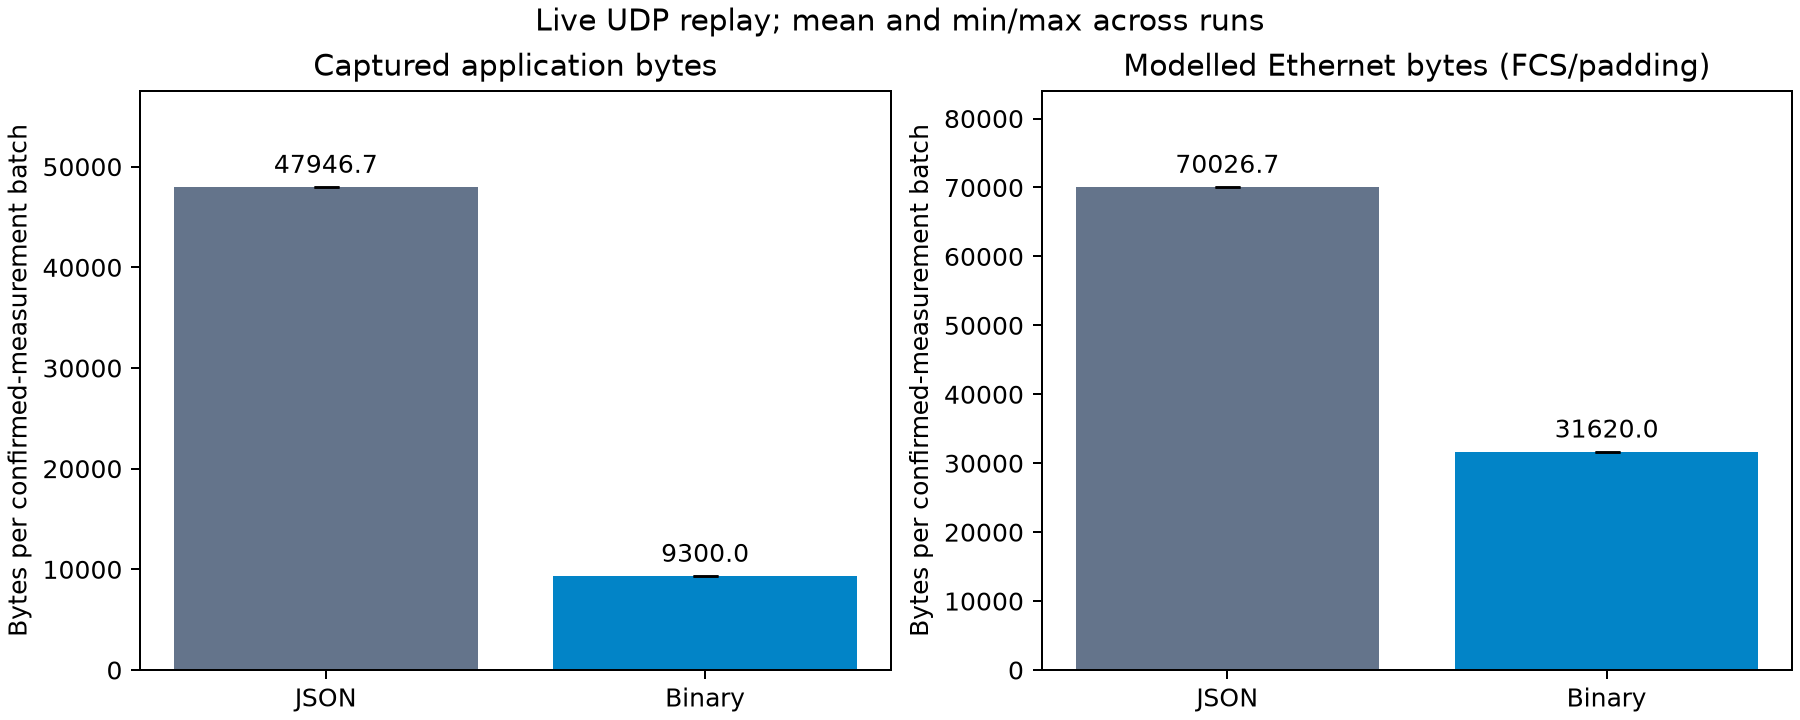
\includegraphics[width=\linewidth]{measurements/live/comparison.png}
\caption{Živé lokálne meranie: priemery a rozsah min./max.; Ethernet je prepočítaný model.}
\end{figure}

Výstupy sú v \texttt{measurements/live/}: \texttt{summary.csv}, \texttt{averages.csv}, manifest vstupov, skutočné \texttt{traffic.pcapng} a prepisy prenesených bajtov. Existujúce výsledky sa neprepisujú. Nový beh:
\begin{quote}\small\singlespacing
\begin{verbatim}
python3 measure_live.py --out measurements/live_novy
\end{verbatim}
\end{quote}
Na meranie cez dve zariadenia podporuje skript externý server, výber IP a rozhrania; presný postup je v \texttt{measurements/LIVE\_MERANIE.txt}. Takýto beh sa v uvedených výsledkoch netvrdí.

\subsection{Porovnanie s existujúcim protokolom CoAP}

CoAP podľa RFC 7252 poskytuje štandardné požiadavky a odpovede nad UDP. Porovnávací model používa CON POST na resource \texttt{/meteo/ID}, osembajtový korelačný token, Uri-Path a Content-Format options; server reaguje piggyback ACK s kódom 2.04 Changed. CoAP-JSON prenáša rovnaké hodnoty ako JSON objekt (Content-Format 50). CoAP-packed používa naše bitové hodnoty ako \texttt{application/octet-stream} (42), nie štandardizovanú schému senzorových dát. Prijímateľ musí poznať formát resource.

\begin{center}\small\singlespacing
\begin{tabular}{l r r}
\hline Model, 240 potvrdených meraní & L7 [B] & Model Ethernet [B] \\\hline
Vlastný JSON & 47\,777 & 69\,857 \\
Vlastný binárny & 9\,300 & 31\,620 \\
CoAP-JSON & 25\,135 & 48\,655 \\
CoAP-packed & 10\,260 & 33\,780 \\\hline
\end{tabular}\end{center}

\begin{figure}[!htbp]
\centering
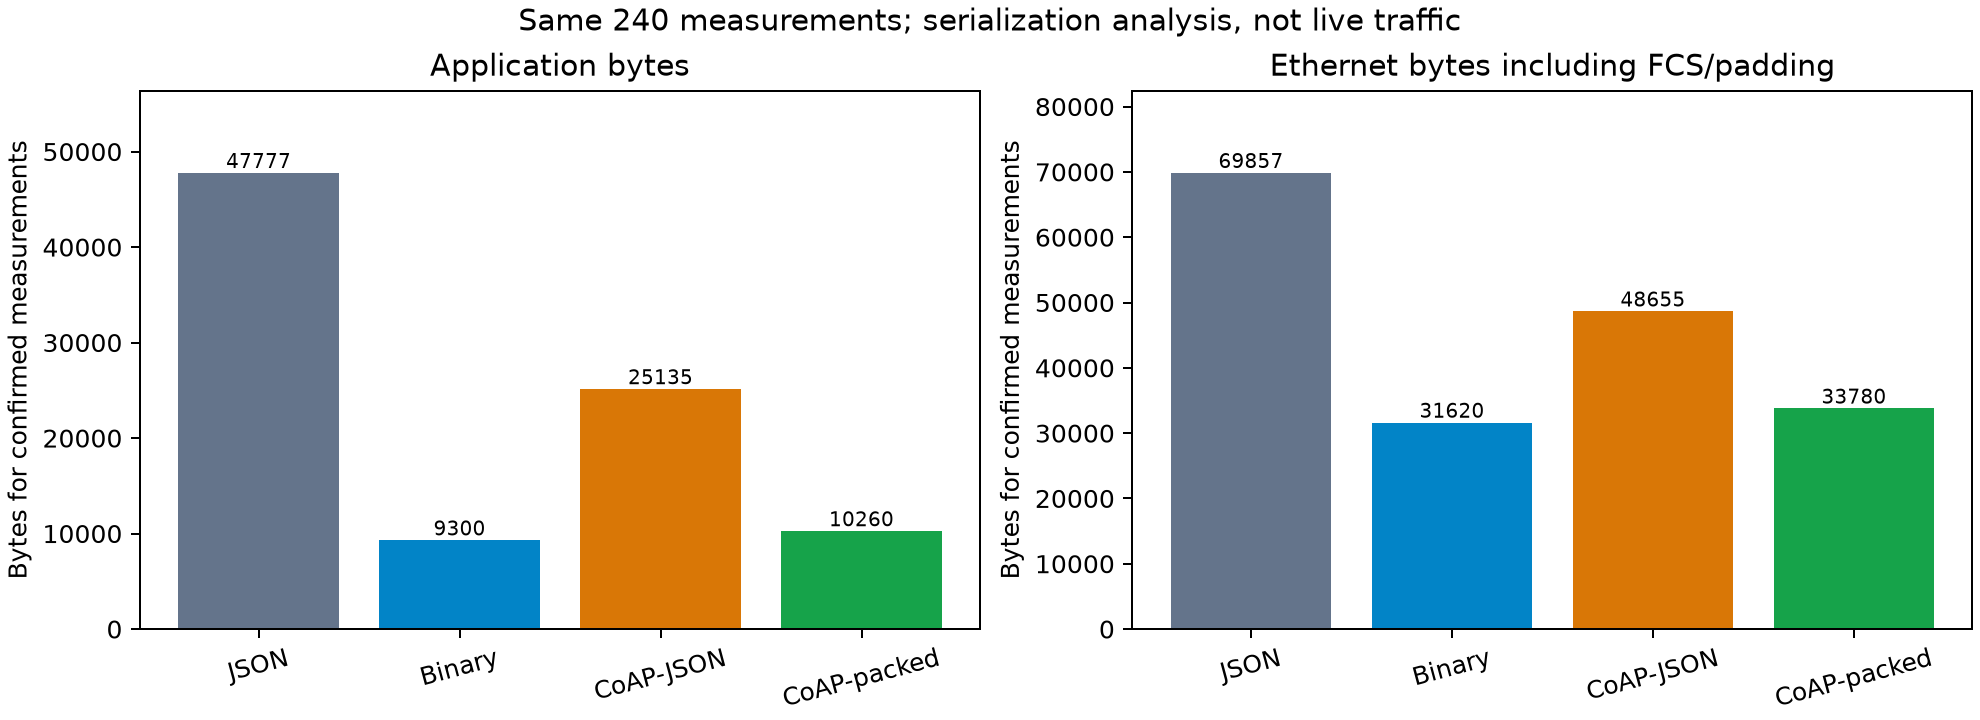
\includegraphics[width=\linewidth]{measurements/comparison.png}
\caption{Model serializácie pri rovnakých vstupoch. Nejde o živé meranie CoAP.}
\end{figure}

CoAP pakety boli vytvorené podľa formátu RFC a dekódované natívnym dissektorom TSharku. \textbf{CoAP server a živý CoAP benchmark zatiaľ nie sú implementované.} CoAP nemá naše registrácie ani aplikačné CRC32 a jeho token slúži na koreláciu, nie na autentifikáciu relácie. Porovnanie preto zahŕňa iba potvrdené merania, nie rovnocennosť všetkých služieb; registrácie sa oddeľujú. Rozdiel medzi CoAP-JSON a CoAP-packed ukazuje vplyv samotnej reprezentácie dát. Veľkosť nášho špecializovaného protokolu nepreukazuje všeobecnú prevahu nad interoperabilným CoAP. SenML (RFC 8428) je príklad štandardnej reprezentácie senzorových údajov, ktorú tento model nepoužíva.

\subsection{Réžia a chybové scenáre}

Binárny ustálený prenos má 5220 B DATA a 4080 B ACK. Zo všetkých 9300 B tvoria zabalené hodnoty iba 1140 B (12,26\,\%); hlavičky DATA a CRC ďalších 4080 B. Minimálna Ethernetová veľkosť preto obmedzuje prínos ďalšieho zmenšovania hodnôt. Výsledky nevyjadrujú spotrebu batérie ani rýchlosť siete.

V \texttt{measurements/summary.csv} sú samostatne modelované scenáre: oprava CRC (4 pakety), päť stratených ACK (7 paketov), tri KEEPALIVE s odpoveďami (6 paketov) a úplné odpojenie (3 sondy). Ich objem sa nemieša s bežným prenosom. Pri JSON ide v prípade straty ACK o model rovnakého scenára, pretože pôvodný JSON program túto funkciu neobsahuje. Správanie aktuálneho binárneho programu pri chybách overujú živé regresné testy.

\section{Zhodnotenie}

Implementácia pokrýva UAT 1--5, nezávislé relácie viacerých senzorov rovnakého typu a lokálne overené obnovovanie po výpadku servera. Bitové polia odstránili textové názvy a desatinné reprezentácie z prenosu. Dissector umožňuje kontrolu obsahu vo Wiresharku. Najväčšou časťou zostávajúcej réžie sú hlavičky a potvrdenia; do budúcnosti prichádza do úvahy ich optimalizácia, dávkovanie meraní a zabezpečenie prenosu. Tieto zmeny by vyžadovali nové merania aj aktualizáciu formátu.

Lokálne testy a loopback meranie nenahrádzajú fyzickú prezentáciu na dvoch zariadeniach. Otvorené zostáva potvrdenie výkladu klientskeho časovača, živé porovnanie s CoAP a automatické riešenie vyčerpania 32-bitovej sekvencie. Protokol neobsahuje kryptografické zabezpečenie a nie je prezentovaný ako produkčne nasadený systém.

\section{Zdroje}
\begin{itemize}
\item RFC 7252: \emph{The Constrained Application Protocol (CoAP)}. \url{https://www.rfc-editor.org/rfc/rfc7252.html}
\item RFC 8428: \emph{Sensor Measurement Lists (SenML)}. \url{https://www.rfc-editor.org/rfc/rfc8428.html}
\item Wireshark Developer's Guide, Lua API. \url{https://www.wireshark.org/docs/wsdg_html_chunked/wsluarm.html}
\end{itemize}

\clearpage
\appendix
\section{Príloha A: Edukatívne zhodnotenie}

Pri riešení projektu som sa naučila navrhovať vlastný aplikačný protokol a prepájať jeho špecifikáciu s implementáciou. Práca s UDP mi ukázala, že potvrdenie, opakovanie, identifikáciu relácie aj kontrolu dostupnosti musí zabezpečiť aplikácia. Pri binárnom formáte som si precvičila výpočet potrebného počtu bitov, kódovanie desatinných hodnôt a poradie bajtov. Dôležité bolo rozlišovať medzi náhodným poškodením dát a bezpečnosťou komunikácie, ktorú samotné CRC neposkytuje.

Vlákna a fronty mi pomohli pochopiť nezávislé spracovanie viacerých senzorov. Regresné testy ukázali význam chybových vstupov, starých tokenov a reštartov, nielen úspešného prenosu. Pri meraní som sa naučila oddeľovať skutočný zachyt od modelu a započítavať aj nižšie sieťové vrstvy. Wireshark a Lua dissector umožnili overiť, čo sa skutočne prenáša.

Tieto skúsenosti môžem využiť pri ďalšom štúdiu sietí, operačných systémov a distribuovaných aplikácií. V praxi mi pomôžu pri diagnostike komunikácie, tvorbe testov a písaní presnej dokumentácie. Zároveň som si uvedomila, že zrozumiteľné výsledky a reprodukovateľný postup sú rovnako dôležité ako funkčný kód.

\end{document}
